\lstset{basicstyle=\ttfamily\small}

\begin{enumerate}[label=\thesubsection.\arabic*, ref=\thesubsection.\theenumi]

%---------------------------------------------------------------------
\item A day can only be cloudy or sunny. The probability of a day being
cloudy is $0.5$, independent of the condition on other days. What is the
probability that in any given four days, there will be three cloudy days
and one sunny day?
\hfill (CS2 2026)
\begin{multicols}{4}
\begin{enumerate}[label=\roman*)]
  \item $\frac{1}{4}$
  \item $\frac{3}{4}$
  \item $\frac{2}{3}$
  \item $\frac{3}{8}$
\end{enumerate}
\end{multicols}
\solution
\begin{table}[H]
\centering
\begin{tabular}{|c|l|c|}
\hline
\textbf{Variable} & \textbf{Description} & \textbf{Value} \\
\hline
$X_i$ & $1$ if day $i$ is cloudy, $0$ if sunny & $\cbrak{0,1}$ \\
$p$ & $\pr{X_i = 1}$ & $0.5$ \\
$q$ & $\pr{X_i = 0} = 1 - p$ & $0.5$ \\
$Y$ & $X_1 + X_2 + X_3 + X_4$ & $\cbrak{0,\dots,4}$ \\
\hline
\end{tabular}
\caption{Variables}
\label{tab:q3vars}
\end{table}
From \eqref{eq:ztrans-bern}, the Z-transform of each day is
\begin{align}
M_{X_i}(z) = q + p\, z^{-1} = \frac{1}{2} + \frac{1}{2} z^{-1}
\label{eq:q3-day}
\end{align}
upon substituting from \tabref{tab:q3vars}. Since the days are
independent, from \eqref{eq:ztrans-prod} and \eqref{eq:q3-day},
\begin{align}
M_Y(z) &= \prod_{i=1}^{4} M_{X_i}(z) = \brak{\frac{1}{2} + \frac{1}{2} z^{-1}}^{4}
= \frac{1}{16}\brak{1 + z^{-1}}^{4} \\
&= \frac{1}{16}\brak{1 + 4z^{-1} + 6z^{-2} + 4z^{-3} + z^{-4}} \\
&= \frac{1}{16} + \frac{4}{16} z^{-1} + \frac{6}{16} z^{-2}
+ \frac{4}{16} z^{-3} + \frac{1}{16} z^{-4}
\label{eq:q3-MY}
\end{align}
Comparing \eqref{eq:q3-MY} with \eqref{eq:ztrans-def}, $p_Y(k)$ is the
coefficient of $z^{-k}$, so
\begin{align}
p_Y(3) = \frac{4}{16} = \frac{1}{4}
\end{align}
This agrees with \eqref{eq:binom-pmf}:
$\binom{4}{3}\brak{0.5}^{3}\brak{0.5}^{1} = \frac{1}{4}$. The answer is
option i).

The following code verifies the solution and generates \figref{fig:q3-pmf}.
\begin{lstlisting}
codes/gate_cs2_q3.py
\end{lstlisting}
\begin{figure}[H]
\centering
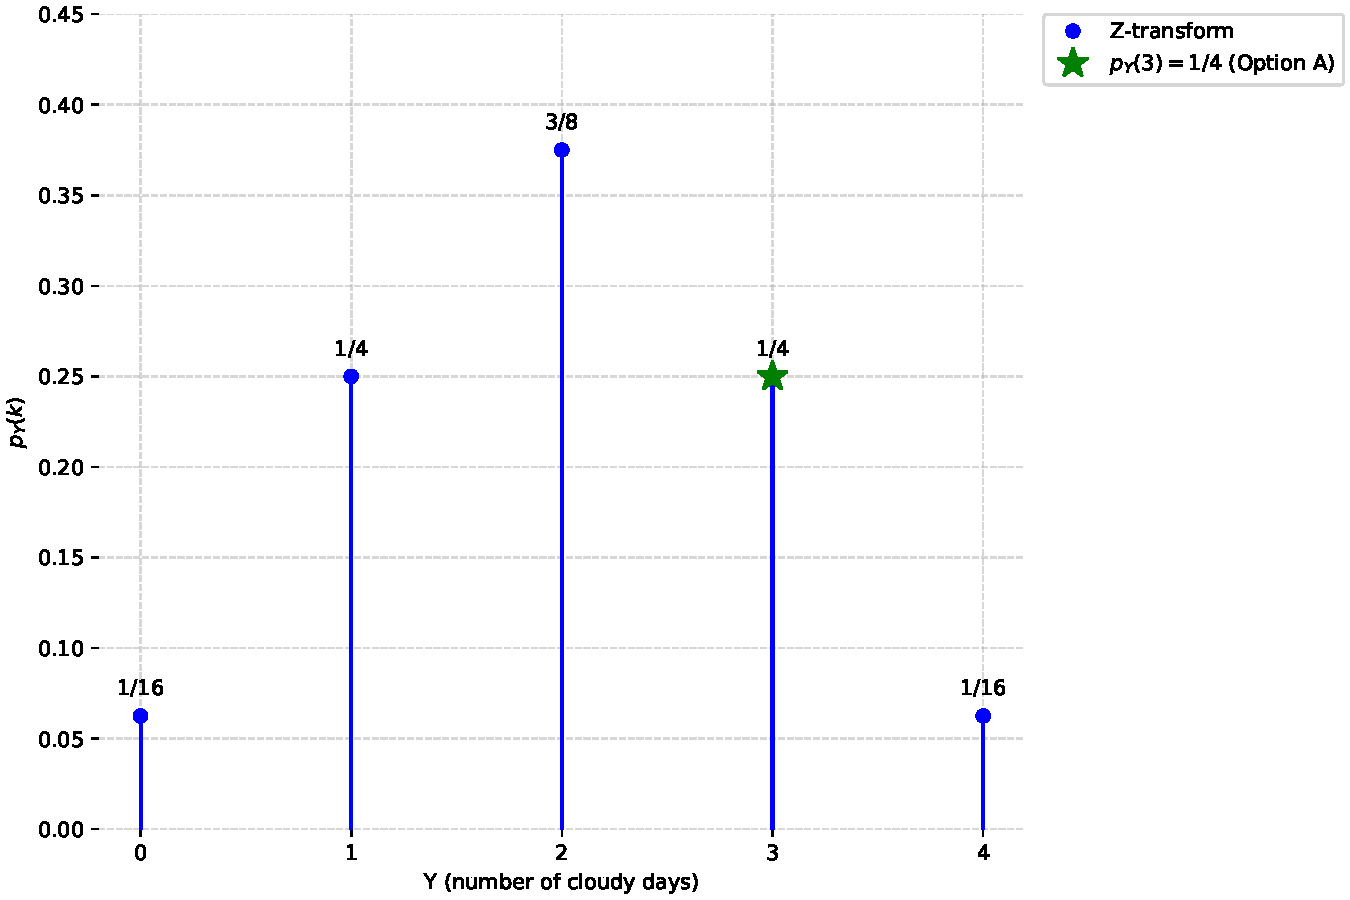
\includegraphics[width=0.9\columnwidth]{figs/pmf.pdf}
\caption{PMF of the number of cloudy days}
\label{fig:q3-pmf}
\end{figure}

%---------------------------------------------------------------------
\item The values of Stock A and Stock B on a particular day are Rs.~50 and
Rs.~80, respectively. An investor invests Rs.~100 in Stock A and Rs.~80 in
Stock B. He sells all the stocks the next day when the value of Stock A is
Rs.~55 and Stock B is Rs.~70. The profit made by the investor is
Rs.~\underline{\hspace{1.5cm}}
\hfill (CS2 2026)
\begin{multicols}{4}
\begin{enumerate}[label=\roman*)]
  \item $0$
  \item $5$
  \item $10$
  \item $20$
\end{enumerate}
\end{multicols}
\solution The number of shares bought is
\begin{align}
\text{Stock A}: \frac{100}{50} = 2, \qquad \text{Stock B}: \frac{80}{80} = 1
\end{align}
and their value the next day is
\begin{align}
2 \times 55 + 1 \times 70 = 180
\end{align}
so the profit is $180 - \brak{100 + 80} = 0$. The answer is option i).

The following code verifies the solution.
\begin{lstlisting}
codes/stock.c
\end{lstlisting}

%---------------------------------------------------------------------
\item An unbiased six-faced dice whose faces are marked with numbers 1, 2,
3, 4, 5, and 6 is rolled twice in succession and the number on the top face
is recorded each time. The probability that the sum of the two recorded
numbers is a prime number is \underline{\hspace{1.5cm}}
\hfill (CS2 2026)
\begin{multicols}{4}
\begin{enumerate}[label=\roman*)]
  \item $\frac{3}{36}$
  \item $\frac{13}{36}$
  \item $\frac{15}{36}$
  \item $\frac{19}{36}$
\end{enumerate}
\end{multicols}
\solution Let $X_1, X_2$ be the two numbers and $S = X_1 + X_2$. From
\eqref{eq:ztrans-die}, the Z-transform of each roll is
\begin{align}
M_{X_i}(z) = \frac{1}{6}\brak{z^{-1} + z^{-2} + z^{-3} + z^{-4} + z^{-5} + z^{-6}}
\label{eq:q10-die}
\end{align}
The two rolls are independent, so from \eqref{eq:ztrans-prod} and
\eqref{eq:q10-die},
\begin{align}
M_S(z) &= M_{X_1}(z)\, M_{X_2}(z)
= \frac{1}{36}\brak{z^{-1} + z^{-2} + \dots + z^{-6}}^{2} \\
&= \frac{1}{36}\big(z^{-2} + 2z^{-3} + 3z^{-4} + 4z^{-5} + 5z^{-6} + 6z^{-7}
\nonumber \\
&\qquad + 5z^{-8} + 4z^{-9} + 3z^{-10} + 2z^{-11} + z^{-12}\big)
\label{eq:q10-MS}
\end{align}
Comparing \eqref{eq:q10-MS} with \eqref{eq:ztrans-def}, $p_S(k)$ is the
coefficient of $z^{-k}$, which agrees with \eqref{eq:dice-sum-pmf}.
\begin{table}[H]
\centering
\begin{tabular}{|c|ccccccccccc|}
\hline
$k$ & 2 & 3 & 4 & 5 & 6 & 7 & 8 & 9 & 10 & 11 & 12 \\
\hline
$36\, p_S(k)$ & 1 & 2 & 3 & 4 & 5 & 6 & 5 & 4 & 3 & 2 & 1 \\
\hline
\end{tabular}
\caption{Coefficients of $M_S(z)$}
\label{tab:q10-pmf}
\end{table}
The primes in $\cbrak{2, \dots, 12}$ are $2, 3, 5, 7, 11$. From
\tabref{tab:q10-pmf},
\begin{align}
\pr{S \text{ prime}} &= p_S(2) + p_S(3) + p_S(5) + p_S(7) + p_S(11) \\
&= \frac{1 + 2 + 4 + 6 + 2}{36} = \frac{15}{36}
\end{align}
The answer is option iii).

The following code verifies the solution by simulation and generates \figref{fig:q10}.
\begin{lstlisting}
codes/dice_sum.py
\end{lstlisting}
\begin{figure}[H]
\centering
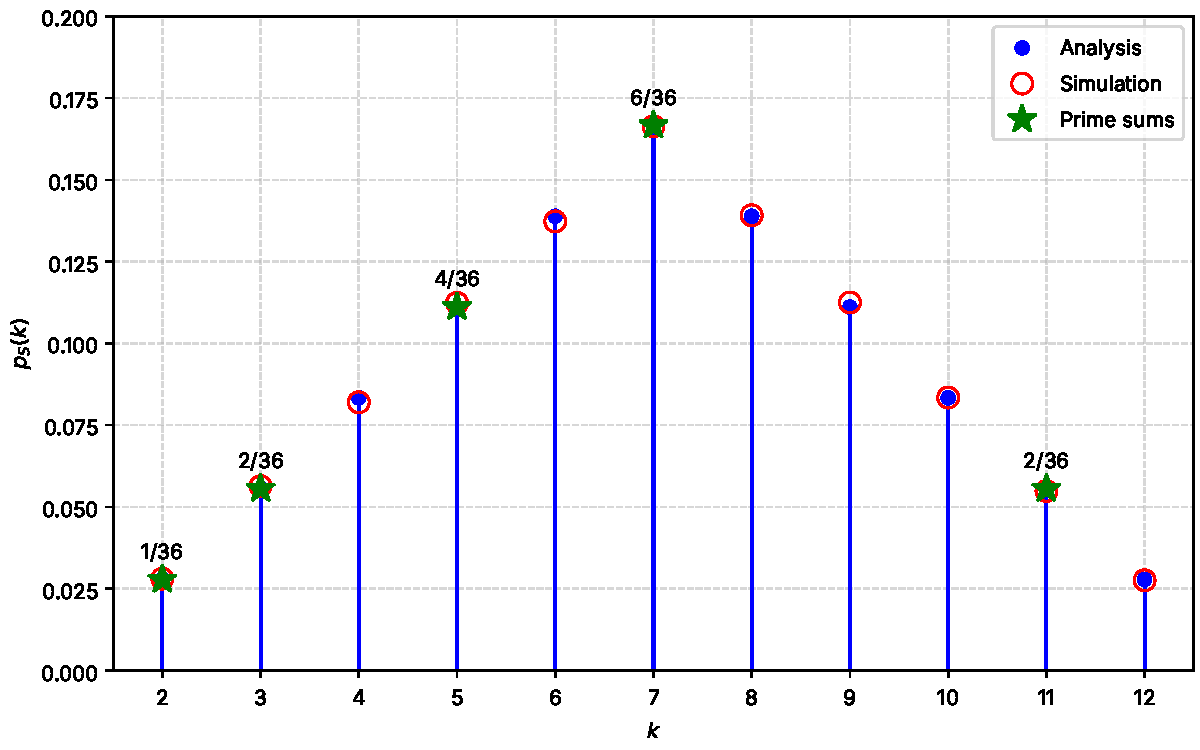
\includegraphics[width=0.85\columnwidth]{figs/dice_sum.pdf}
\caption{PMF of the sum of two dice, with the prime sums marked}
\label{fig:q10}
\end{figure}

%---------------------------------------------------------------------
\item The probability density function $f(x)$ of a random variable $X$
which takes real values is
\begin{align}
f(x) = \frac{1}{3\sqrt{2\pi}}\exp\brak{-\frac{x^2}{18}}, \quad
x \in \brak{-\infty, +\infty}
\label{eq:q14-pdf}
\end{align}
Which one of the following statements is correct about the random
variable $X$?
\hfill (CS2 2026)
\begin{enumerate}[label=\roman*)]
  \item $X$ is an exponential random variable
  \item $X$ is a normal random variable
  \item $X$ is a Poisson random variable
  \item $X$ is a uniform random variable
\end{enumerate}
\solution \textbf{Option ii) is true: $X$ is a normal random variable.}
Comparing \eqref{eq:q14-pdf} with \eqref{eq:gauss-pdf},
\begin{align}
\mu = 0, \quad 2\sigma^2 = 18 \implies \sigma = 3
\end{align}
so $X \sim \gauss{0}{9}$.

\textbf{The other options are false:}
\begin{itemize}
  \item \textbf{i) Exponential.} From \eqref{eq:exp-pdf}, an exponential
  PDF is $0$ for all $x < 0$. But \eqref{eq:q14-pdf} is positive for every
  real $x$, for example
  \begin{align}
  f(-3) = \frac{1}{3\sqrt{2\pi}} e^{-1/2} > 0
  \end{align}
  It is also symmetric, $f(-x) = f(x)$, while an exponential PDF is
  decreasing from $x = 0$.
  \item \textbf{iii) Poisson.} From \eqref{eq:poisson-pmf}, a Poisson
  random variable is discrete: it takes only the values $0, 1, 2, \dots$
  and is described by a PMF. But $X$ takes all real values in
  $\brak{-\infty, \infty}$, including negative and non-integer values,
  and is described by a PDF.
  \item \textbf{iv) Uniform.} From \eqref{eq:unif-pdf}, a uniform PDF is
  constant on $[a, b]$ and zero outside it. But \eqref{eq:q14-pdf} changes
  with $x$, for example
  \begin{align}
  f(0) = \frac{1}{3\sqrt{2\pi}} \ne f(3) = \frac{1}{3\sqrt{2\pi}} e^{-1/2}
  \end{align}
  and it is never zero.
\end{itemize}
The answer is option ii).

The following code compares the numerical PDF of $\gauss{0}{9}$ samples with \eqref{eq:q14-pdf} in \figref{fig:q14}.
\begin{lstlisting}
codes/gauss.py
\end{lstlisting}
\begin{figure}[H]
\centering
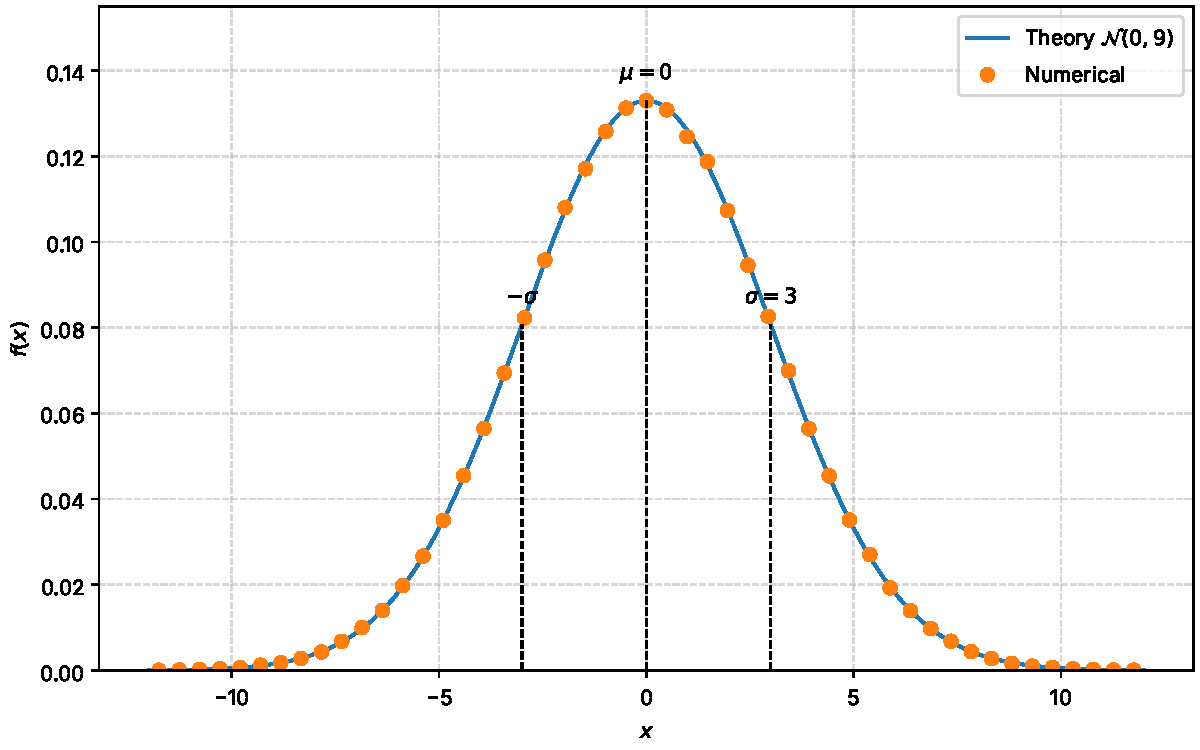
\includegraphics[width=0.85\columnwidth]{figs/gauss.pdf}
\caption{Numerical PDF vs $\gauss{0}{9}$}
\label{fig:q14}
\end{figure}

%---------------------------------------------------------------------
\item Consider the following three ANSI-C programs, P1, P2, and P3.
\hfill (CS2 2026)

\noindent
\begin{minipage}[t]{0.32\linewidth}
\centering P1
\begin{lstlisting}[language=C]
#include <stdio.h>
int a=5;
int main(){
  int a=7;
  return(0);
}
\end{lstlisting}
\end{minipage}\hfill
\begin{minipage}[t]{0.32\linewidth}
\centering P2
\begin{lstlisting}[language=C]
#include <stdio.h>
int main(){
  int a=5;
  int a=7;
  return(0);
}
\end{lstlisting}
\end{minipage}\hfill
\begin{minipage}[t]{0.32\linewidth}
\centering P3
\begin{lstlisting}[language=C]
#include <stdio.h>
int main(){
  int a=5;
  float a=7;
  return(0);
}
\end{lstlisting}
\end{minipage}

Which one of the following statements is true?
\begin{enumerate}[label=\roman*)]
  \item Only P1 will compile without any error
  \item Only P2 will compile without any error
  \item Only P3 will compile without any error
  \item All three programs P1, P2, and P3 will compile without any error
\end{enumerate}
\solution From \ref{fm:c-scope}, a scope is the region of code in which a
name is visible. Everything outside all functions is the \emph{file
scope}, and each pair of braces \texttt{\{ \}} starts a new \emph{block
scope}.
\begin{itemize}
  \item \textbf{P1 compiles.} \texttt{int a=5;} is outside \texttt{main},
  in file scope, while \texttt{int a=7;} is inside the braces of
  \texttt{main}, in block scope. These are two different variables in two
  different scopes. Inside \texttt{main} the local \texttt{a} hides the
  global one, which is allowed.

  \item \textbf{P2 does not compile: redefinition.} Both
  \texttt{int a=5;} and \texttt{int a=7;} are inside the same braces of
  \texttt{main}, so they are in the same block scope. The compiler would
  have to create two variables with the same name in the same place, and
  then could not tell which one a later use of \texttt{a} refers to. C
  forbids this. Note that \texttt{int a=7;} is a new declaration, not an
  assignment. Writing \texttt{a=7;} instead would compile and simply change
  the value of \texttt{a}. The compiler reports
  \begin{lstlisting}[mathescape=false]
p2.c:5:7: error: redefinition of 'a'
  \end{lstlisting}

  \item \textbf{P3 does not compile: conflicting types.} This is the same
  mistake, declaring \texttt{a} twice in the same block scope, but now
  with different types: first \texttt{int}, then \texttt{float}. A
  variable has exactly one type for its whole lifetime, so \texttt{a}
  cannot be both an \texttt{int} and a \texttt{float}. Changing the type
  does not make it a different variable. The compiler reports
  \begin{lstlisting}[mathescape=false]
p3.c:5:9: error: conflicting types for 'a'; have 'float'
  \end{lstlisting}
\end{itemize}
P1 shows that the same name may be reused in a \emph{different} scope.
P2 and P3 fail because they reuse it in the \emph{same} scope, whatever
the type. The answer is option i).

Compiling the three programs confirms the solution: only P1 compiles.
\begin{lstlisting}
codes/p1.c
codes/p2.c
codes/p3.c
\end{lstlisting}

%---------------------------------------------------------------------
\item Consider the following functions, where $n$ is a positive integer.
\begin{align*}
n^{1/3}, \quad \log(n), \quad \log(n!), \quad 2^{\log(n)}
\end{align*}
Which one of the following options lists the functions in increasing order
of asymptotic growth rate?

\textit{Note:} Assume the base of $\log$ to be $2$.
\hfill (CS2 2026)
\begin{enumerate}[label=\roman*)]
  \item $\log(n),\ n^{1/3},\ 2^{\log(n)},\ \log(n!)$
  \item $n^{1/3},\ \log(n),\ \log(n!),\ 2^{\log(n)}$
  \item $\log(n),\ n^{1/3},\ \log(n!),\ 2^{\log(n)}$
  \item $2^{\log(n)},\ n^{1/3},\ \log(n),\ \log(n!)$
\end{enumerate}
\solution With base 2, $2^{\log(n)} = n$. From \eqref{eq:log-fact},
$\log(n!) = \Theta\brak{n\log(n)}$, so $\log(n!)$ grows at the same rate as
$n\log(n)$ (see \eqref{eq:theta}). It remains to order
$\log(n)$, $n^{1/3}$, $n$ and $n\log(n)$. Here $o$ is little-o from
\eqref{eq:little-o}: $f = o(g)$ means $\frac{f}{g} \to 0$, that is, $f$
grows strictly slower than $g$. From \eqref{eq:growth},
\begin{align}
\log(n) = o\brak{n^{1/3}}, \quad n^{1/3} = o(n), \quad n = o\brak{n\log(n)}
\label{eq:q24-chain}
\end{align}
Each ratio goes to $0$:
\begin{table}[H]
\centering
\begin{tabular}{|c|c|l|}
\hline
\textbf{Statement} & \textbf{Ratio} & \textbf{Why it goes to 0} \\
\hline
$\log(n) = o\brak{n^{1/3}}$ & $\dfrac{\log(n)}{n^{1/3}}$ &
\begin{tabular}[c]{@{}l@{}}a power of $n$ beats a logarithm;\\
at $n = 10^{8}$: $\log(n) \approx 27$, $n^{1/3} \approx 464$\end{tabular} \\
\hline
$n^{1/3} = o(n)$ & $\dfrac{n^{1/3}}{n} = \dfrac{1}{n^{2/3}}$ &
$n^{2/3} \to \infty$ \\
\hline
$n = o\brak{n\log(n)}$ & $\dfrac{n}{n\log(n)} = \dfrac{1}{\log(n)}$ &
$\log(n) \to \infty$ \\
\hline
\end{tabular}
\caption{Ratios in \eqref{eq:q24-chain}}
\end{table}
Chaining \eqref{eq:q24-chain} gives
$\log(n) < n^{1/3} < n < n\log(n)$ in growth rate. Since
$2^{\log(n)} = n$ and $\log(n!) = \Theta\brak{n\log(n)}$, the order is
$\log(n),\ n^{1/3},\ 2^{\log(n)},\ \log(n!)$. The answer is option i).

The following code plots the four functions in \figref{fig:q24}. Note that $n^{1/3}$ overtakes $\log(n)$ only after $n \approx 10^3$.
\begin{lstlisting}
codes/growth.py
\end{lstlisting}
\begin{figure}[H]
\centering
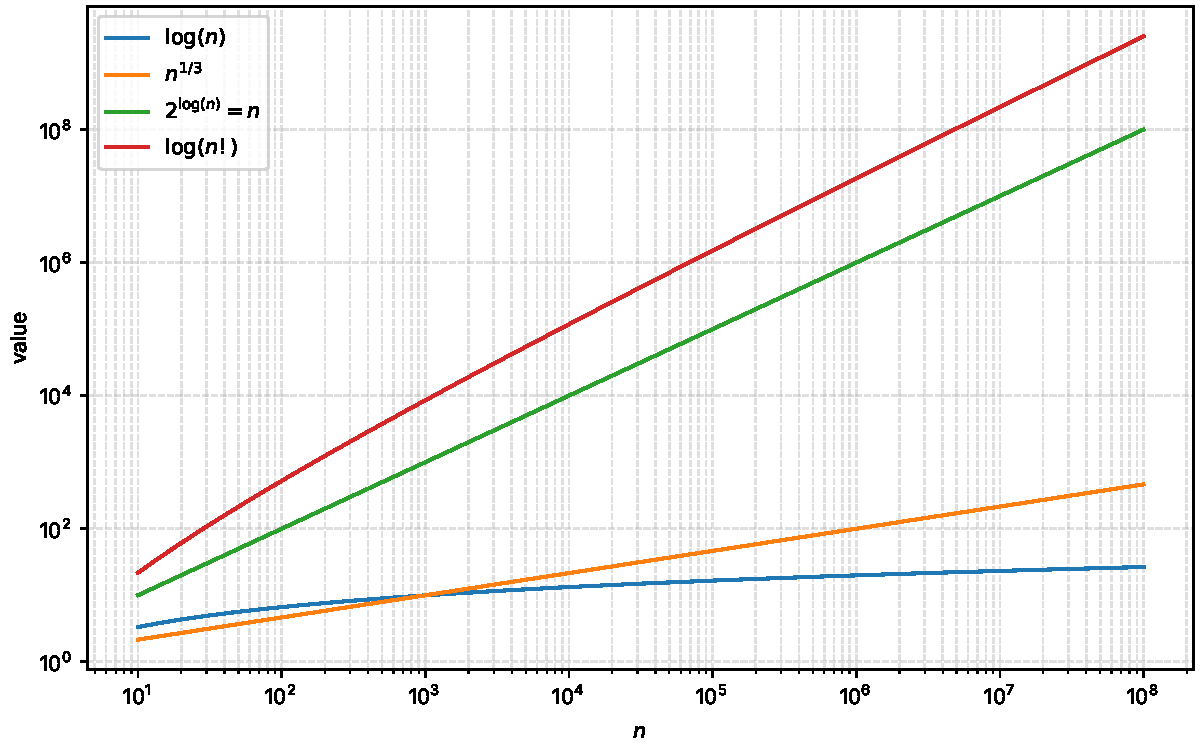
\includegraphics[width=0.85\columnwidth]{figs/growth.pdf}
\caption{Growth of the four functions}
\label{fig:q24}
\end{figure}

%---------------------------------------------------------------------
\item Which of the following can be recurrence relation(s) corresponding to
an algorithm with time complexity $\Theta(n)$?
\hfill (CS2 2026)
\begin{multicols}{2}
\begin{enumerate}[label=\roman*)]
  \item $T(n) = T(n-1) + 1,\ T(1) = 1$
  \item $T(n) = 2T\brak{\frac{n}{2}} + 1,\ T(1) = 1$
  \item $T(n) = 2T\brak{\frac{n}{2}} + n,\ T(1) = 1$
  \item $T(n) = T(n-1) + n,\ T(1) = 1$
\end{enumerate}
\end{multicols}
\solution Each recurrence is turned into a sequence $x[k]$, $k \ge 0$,
and solved with the Z-transform. In each case setting $x[-1] = 0$
reproduces the initial condition, so \eqref{eq:zseq-shift} applies.
\begin{enumerate}[label=\roman*)]
  \item Let $x[k] = T(k+1)$. Then
  \begin{align}
  x[k] = x[k-1] + 1, \quad x[0] = 1
  \end{align}
  Taking the Z-transform using \eqref{eq:zseq-shift} and
  \eqref{eq:zseq-geo} with $a = 1$,
  \begin{align}
  X(z) = z^{-1}X(z) + \frac{1}{1 - z^{-1}}
  \implies X(z) = \frac{1}{\brak{1 - z^{-1}}^{2}}
  \end{align}
  From \eqref{eq:zseq-geo2} with $a = 1$, $x[k] = k + 1$, so
  \begin{align}
  T(n) = x[n-1] = n = \Theta(n)
  \end{align}

  \item Let $n = 2^{k}$ and $x[k] = T\brak{2^{k}}$. Since
  $T\brak{\frac{n}{2}} = x[k-1]$,
  \begin{align}
  x[k] = 2x[k-1] + 1, \quad x[0] = 1
  \end{align}
  Taking the Z-transform,
  \begin{align}
  X(z) = 2z^{-1}X(z) + \frac{1}{1 - z^{-1}}
  \implies X(z) = \frac{1}{\brak{1 - 2z^{-1}}\brak{1 - z^{-1}}}
  \end{align}
  By partial fractions,
  \begin{align}
  X(z) = \frac{2}{1 - 2z^{-1}} - \frac{1}{1 - z^{-1}}
  \end{align}
  so from \eqref{eq:zseq-geo}, $x[k] = 2 \cdot 2^{k} - 1$, and
  \begin{align}
  T(n) = 2n - 1 = \Theta(n)
  \end{align}

  \item With $n = 2^{k}$ and $x[k] = T\brak{2^{k}}$,
  \begin{align}
  x[k] = 2x[k-1] + 2^{k}, \quad x[0] = 1
  \end{align}
  Taking the Z-transform using \eqref{eq:zseq-geo} with $a = 2$,
  \begin{align}
  X(z) = 2z^{-1}X(z) + \frac{1}{1 - 2z^{-1}}
  \implies X(z) = \frac{1}{\brak{1 - 2z^{-1}}^{2}}
  \end{align}
  From \eqref{eq:zseq-geo2} with $a = 2$, $x[k] = (k+1)\,2^{k}$. Since
  $k = \log(n)$,
  \begin{align}
  T(n) = n\brak{\log(n) + 1} = \Theta\brak{n\log(n)}
  \end{align}

  \item Let $x[k] = T(k+1)$. Then
  \begin{align}
  x[k] = x[k-1] + (k+1), \quad x[0] = 1
  \end{align}
  Taking the Z-transform using \eqref{eq:zseq-geo2} with $a = 1$,
  \begin{align}
  X(z) = z^{-1}X(z) + \frac{1}{\brak{1 - z^{-1}}^{2}}
  \implies X(z) = \frac{1}{\brak{1 - z^{-1}}^{3}}
  \end{align}
  From \eqref{eq:zseq-geo3}, $x[k] = \frac{(k+1)(k+2)}{2}$, so
  \begin{align}
  T(n) = x[n-1] = \frac{n(n+1)}{2} = \Theta\brak{n^{2}}
  \end{align}
  which agrees with \eqref{eq:arith-sum}.
\end{enumerate}
Only i) and ii) are $\Theta(n)$, in agreement with the master theorem
\eqref{eq:master}. The answer is options i) and ii).

The following code checks each closed form above against the recurrence and plots $T(n)/n$ in \figref{fig:q25}. It stays bounded only for i) and ii).
\begin{lstlisting}
codes/recurrence.py
\end{lstlisting}
\begin{figure}[H]
\centering
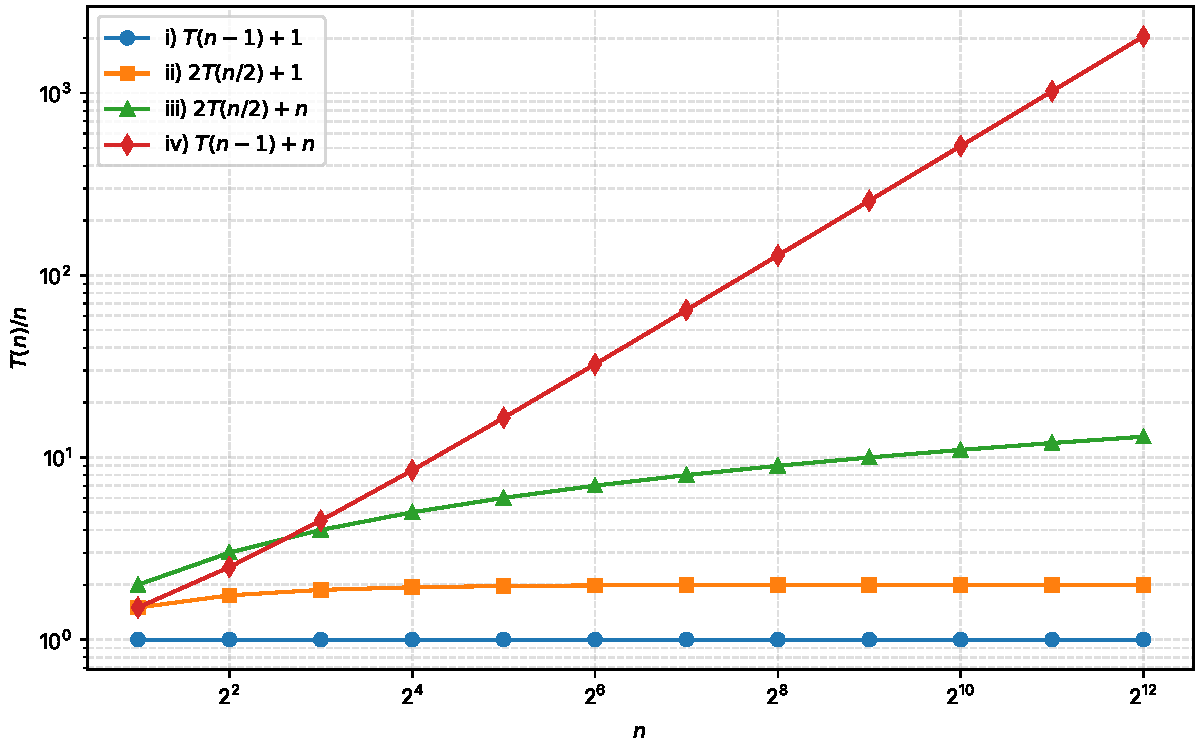
\includegraphics[width=0.85\columnwidth]{figs/recurrence.pdf}
\caption{$T(n)/n$ for the four recurrences}
\label{fig:q25}
\end{figure}

%---------------------------------------------------------------------
\item Let $R$ be a binary relation on the set $\cbrak{1, 2, \dots, 10}$,
where $(x, y) \in R$ if the product of $x$ and $y$ is square of an integer.
Which of the following properties is/are satisfied by $R$?
\hfill (CS2 2026)
\begin{multicols}{4}
\begin{enumerate}[label=\roman*)]
  \item Reflexive
  \item Symmetric
  \item Transitive
  \item Antisymmetric
\end{enumerate}
\end{multicols}
\solution Checking each property against
\eqref{eq:rel-ref}--\eqref{eq:rel-anti}:
\begin{itemize}
  \item Reflexive: $x \cdot x = x^2$.
  \item Symmetric: $xy = yx$.
  \item Transitive: if $xy = a^2$ and $yz = b^2$, then
  \begin{align}
  xz \cdot y^2 = a^2 b^2 \implies xz = \brak{\frac{ab}{y}}^2
  \end{align}
  An integer that is the square of a rational is the square of an integer,
  so $(x, z) \in R$.
  \item Not antisymmetric: $(1, 4), (4, 1) \in R$ since $1 \times 4 = 2^2$,
  but $1 \ne 4$.
\end{itemize}
The answer is options i), ii) and iii).

The following code checks all four properties and draws $R$ in \figref{fig:q26}.
\begin{lstlisting}
codes/relation.py
\end{lstlisting}
\begin{figure}[H]
\centering
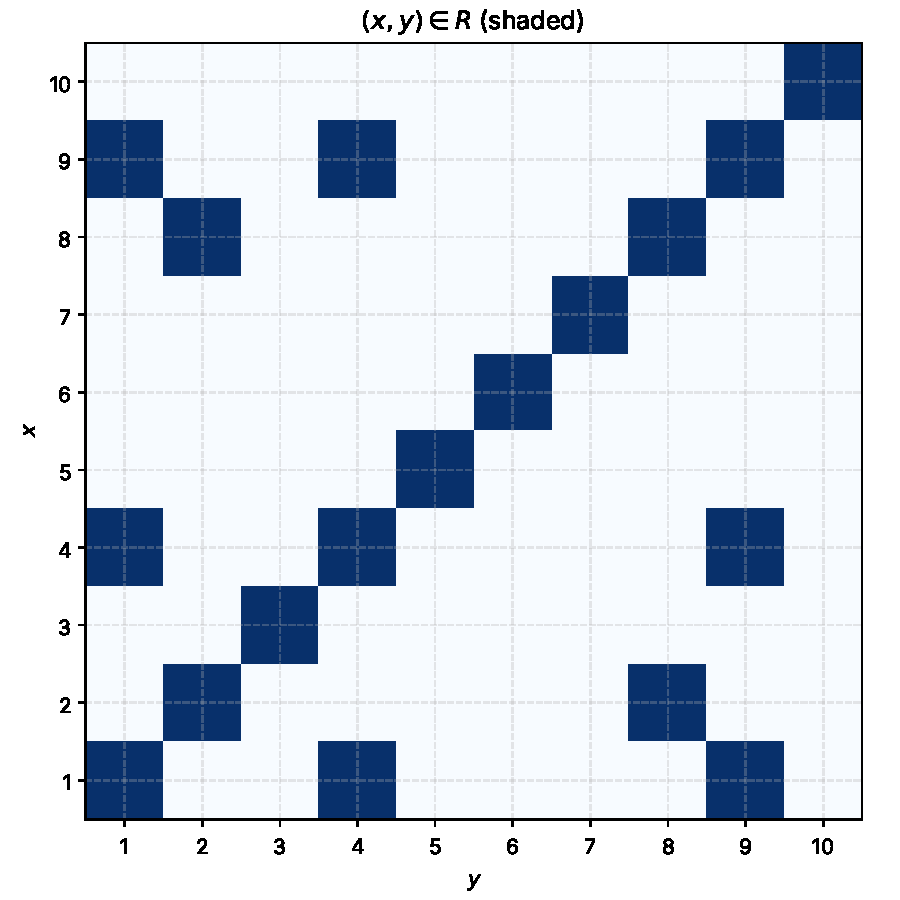
\includegraphics[width=0.85\columnwidth]{figs/relation.pdf}
\caption{The relation $R$ on $\cbrak{1, \dots, 10}$}
\label{fig:q26}
\end{figure}

%---------------------------------------------------------------------
\item For a real number $a$, let
\begin{align}
I(a) = \int_{-1}^{1}\brak{3x^2 - ax + 1}\, dx .
\end{align}
Which of the following statements is/are true?
\hfill (CS2 2026)
\begin{enumerate}[label=\roman*)]
  \item The value of $I(a)$ is independent of the value of $a$
  \item The value of $I(a)$ can vary with the value of $a$
  \item There exists $a \in \brak{-\infty, +\infty}$ such that $I(a)$ is a
  positive real number
  \item There exists $a \in \brak{-\infty, +\infty}$ such that $I(a)$ is a
  negative real number
\end{enumerate}
\solution Since $ax$ is odd, from \eqref{eq:odd-int} and
\eqref{eq:power-rule},
\begin{align}
I(a) = \Big[x^3 + x\Big]_{-1}^{1} - a \cdot 0 = 2 - (-2) = 4
\end{align}
for every $a$. So i) and iii) are true and ii) and iv) are false. The answer
is options i) and iii).

The following code evaluates $I(a)$ numerically in \figref{fig:q27}.
\begin{lstlisting}
codes/integral.py
\end{lstlisting}
\begin{figure}[H]
\centering
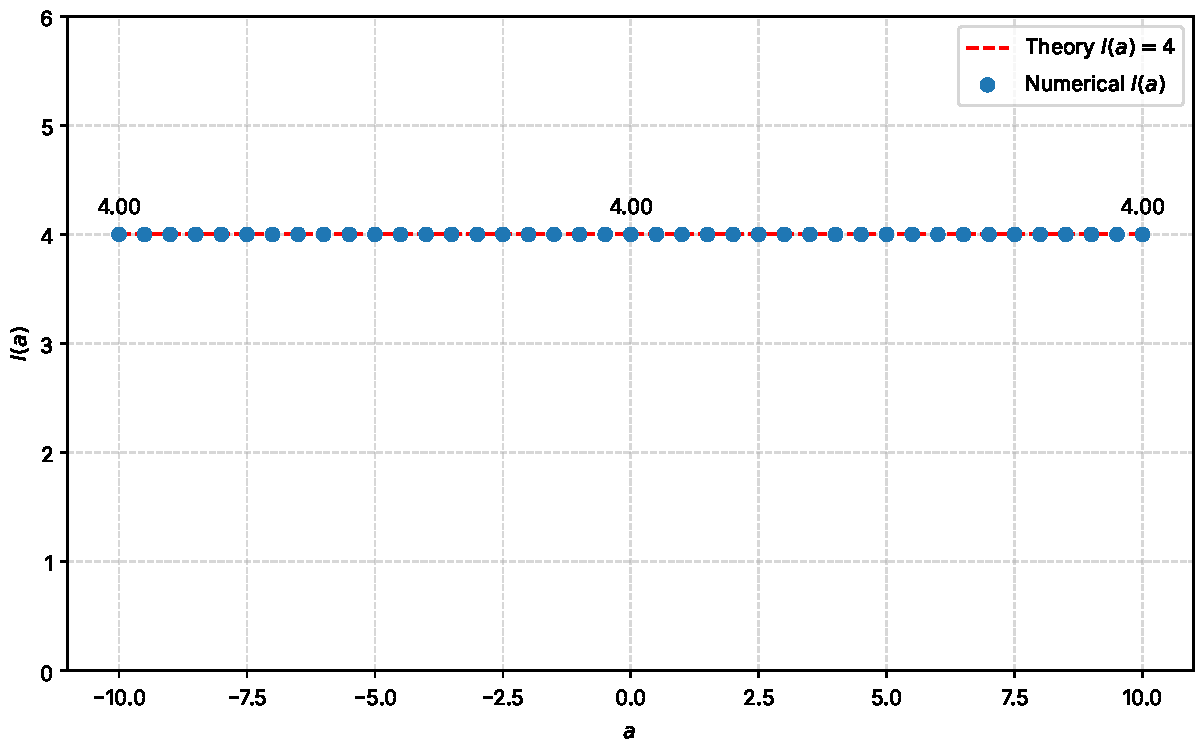
\includegraphics[width=0.85\columnwidth]{figs/integral.pdf}
\caption{$I(a)$ for $-10 \le a \le 10$}
\label{fig:q27}
\end{figure}

%---------------------------------------------------------------------
\item In a system, numbers are represented using 4-bit two's complement
form. Consider four numbers $N_1 = 1011$, $N_2 = 1101$, $N_3 = 1010$ and
$N_4 = 1001$ in the system. Which of the following operations will result
in arithmetic overflow?
\hfill (CS2 2026)
\begin{multicols}{4}
\begin{enumerate}[label=\roman*)]
  \item $N_1 + N_2$
  \item $N_2 + N_3$
  \item $N_3 - N_4$
  \item $N_1 + N_4$
\end{enumerate}
\end{multicols}
\solution From \eqref{eq:twos-val},
\begin{align}
N_1 = -5, \quad N_2 = -3, \quad N_3 = -6, \quad N_4 = -7
\end{align}
and from \eqref{eq:twos-range} the range is $-8 \le x \le 7$.
\begin{table}[H]
\centering
\begin{tabular}{|c|c|c|c|}
\hline
\textbf{Option} & \textbf{Operation} & \textbf{Result} & \textbf{Overflow?} \\
\hline
i) & $-5 + (-3)$ & $-8$ & No \\
ii) & $-3 + (-6)$ & $-9$ & Yes \\
iii) & $-6 - (-7)$ & $1$ & No \\
iv) & $-5 + (-7)$ & $-12$ & Yes \\
\hline
\end{tabular}
\caption{Operations}
\end{table}
The answer is options ii) and iv).

The following code verifies the solution.
\begin{lstlisting}
codes/twos.c
\end{lstlisting}

%---------------------------------------------------------------------
\item The keys 5, 28, 19, 15, 26, 33, 12, 17, 10 are inserted into a hash
table using the hash function $h(k) = k \bmod 9$. The collisions are
resolved by chaining. After all the keys are inserted, the length of the
longest chain is \underline{\hspace{1.5cm}}. (\textit{answer in integer})
\hfill (CS2 2026)

\solution From \eqref{eq:hash} with $m = 9$:
\begin{table}[H]
\centering
\begin{tabular}{|c|ccccccccc|}
\hline
$k$ & 5 & 28 & 19 & 15 & 26 & 33 & 12 & 17 & 10 \\
\hline
$h(k)$ & 5 & 1 & 1 & 6 & 8 & 6 & 3 & 8 & 1 \\
\hline
\end{tabular}
\caption{Hash values}
\end{table}
Slot 1 holds $28, 19, 10$, so the longest chain has length $3$.

The following code builds the chains and draws them in \figref{fig:q30}.
\begin{lstlisting}
codes/hash.py
\end{lstlisting}
\begin{figure}[H]
\centering
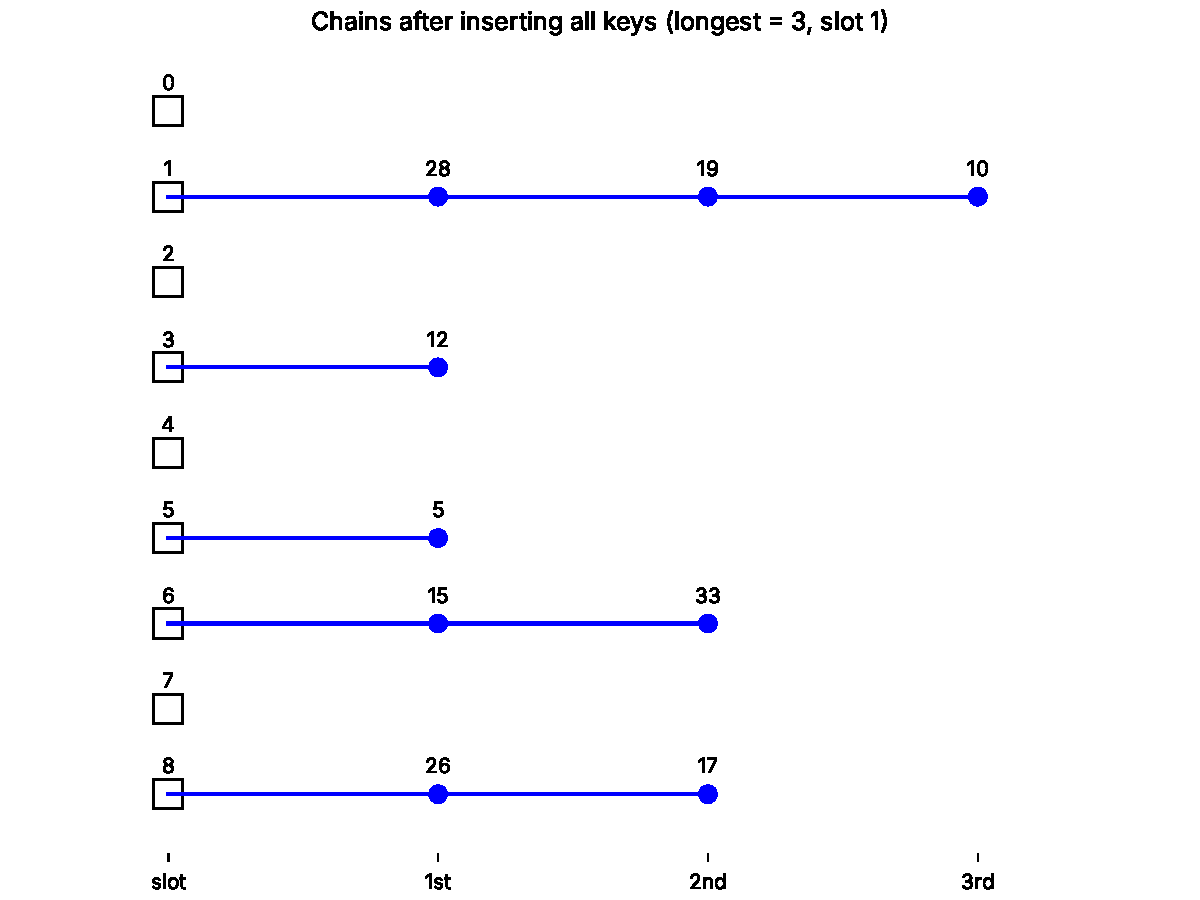
\includegraphics[width=0.85\columnwidth]{figs/hash.pdf}
\caption{Chains in the hash table}
\label{fig:q30}
\end{figure}

%---------------------------------------------------------------------
\item Consider the system of linear equations given below.
\begin{align}
ax + y &= b \\
16x + ay &= 24
\end{align}
Suppose the values of $a$ and $b$ are chosen such that the system of linear
equations produce multiple solutions. Then the product of $a$ and $b$ is
\underline{\hspace{1.5cm}}. (\textit{answer in integer})
\hfill (CS2 2026)

\solution This is solved using row reduction \ref{fm:row-reduce}, the characteristic equation
\eqref{eq:chareq} and the Cayley-Hamilton theorem \eqref{eq:cayley}.
The system is $\vec{A}\vec{x} = \vec{c}$ with augmented matrix
\begin{align}
\myvec{\vec{A} & \vec{c}} = \myvec{a & 1 & b \\ 16 & a & 24}
\label{eq:q31-aug}
\end{align}
If $a = 0$, the equations are $y = b$ and $16x = 24$, which have the unique
solution $\brak{\frac{3}{2}, b}$. So $a \ne 0$, and using \eqref{eq:row-op}
with $R_2 \leftarrow aR_2 - 16R_1$,
\begin{align}
\myvec{a & 1 & b \\ 16 & a & 24}
\xleftrightarrow{R_2 \leftarrow aR_2 - 16R_1}
\myvec{a & 1 & b \\ 0 & a^2 - 16 & 24a - 16b}
\label{eq:q31-red}
\end{align}
From \ref{fm:row-reduce}, there are infinitely many solutions only if the
second row of \eqref{eq:q31-red} is entirely zero:
\begin{align}
a^2 - 16 &= 0
\label{eq:q31-c1} \\
24a - 16b &= 0
\label{eq:q31-c2}
\end{align}

\textbf{Solving \eqref{eq:q31-c1} with the characteristic equation.} Let
\begin{align}
\vec{N} = \myvec{0 & 1 \\ 16 & 0}
\end{align}
From \eqref{eq:chareq}, its characteristic equation is
\begin{align}
f\brak{\lambda} = \mydet{-\lambda & 1 \\ 16 & -\lambda}
= \lambda^2 - 16 = 0 \implies \lambda = \pm 4
\label{eq:q31-char}
\end{align}
and from \eqref{eq:cayley}, $\vec{N}^2 - 16\vec{I} = \vec{0}$. Since
$a^2 - 16 = f\brak{-a}$, \eqref{eq:q31-c1} holds exactly when $-a$ is a root
of \eqref{eq:q31-char}, so $a = \pm 4$.

\textbf{Solving \eqref{eq:q31-c2}.} $b = \frac{24a}{16} = \frac{3a}{2}$, so
\begin{align}
a = 4 &\implies b = 6 \\
a = -4 &\implies b = -6
\end{align}

\textbf{Checking by row reduction.} For $a = 4$, $b = 6$,
\begin{align}
\myvec{4 & 1 & 6 \\ 16 & 4 & 24}
\xleftrightarrow{R_2 \leftarrow R_2 - 4R_1}
\myvec{4 & 1 & 6 \\ 0 & 0 & 0}
\xleftrightarrow{R_1 \leftarrow \frac{R_1}{4}}
\myvec{1 & \frac{1}{4} & \frac{3}{2} \\ 0 & 0 & 0}
\end{align}
The zero row leaves $y$ free:
\begin{align}
x = \frac{3}{2} - \frac{1}{4}y \implies
\vec{x} = \myvec{\frac{3}{2} \\ 0} + y\myvec{-\frac{1}{4} \\ 1}
\label{eq:q31-sol1}
\end{align}
For $a = -4$, $b = -6$,
\begin{align}
\myvec{-4 & 1 & -6 \\ 16 & -4 & 24}
\xleftrightarrow{R_2 \leftarrow R_2 + 4R_1}
\myvec{-4 & 1 & -6 \\ 0 & 0 & 0}
\xleftrightarrow{R_1 \leftarrow -\frac{R_1}{4}}
\myvec{1 & -\frac{1}{4} & \frac{3}{2} \\ 0 & 0 & 0}
\end{align}
so
\begin{align}
\vec{x} = \myvec{\frac{3}{2} \\ 0} + y\myvec{\frac{1}{4} \\ 1}
\label{eq:q31-sol2}
\end{align}
Both cases have infinitely many solutions, and in both
\begin{align}
ab = 24
\end{align}

The following code draws the solution
lines \eqref{eq:q31-sol1} and \eqref{eq:q31-sol2} in \figref{fig:q31}.
\begin{lstlisting}
codes/lines.py
\end{lstlisting}
\begin{figure}[H]
\centering
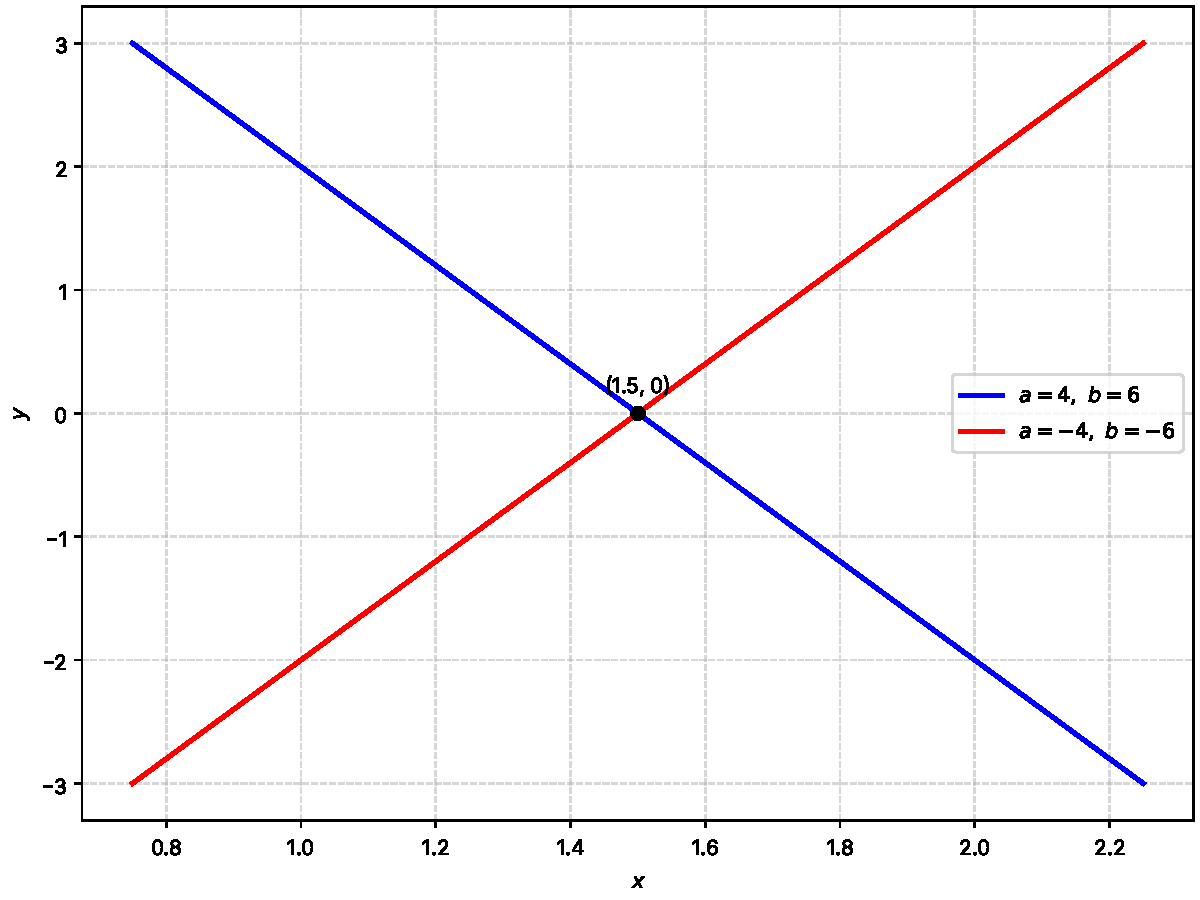
\includegraphics[width=0.85\columnwidth]{figs/lines.pdf}
\caption{Solution lines for $\brak{a, b} = \brak{4, 6}$ and $\brak{-4, -6}$}
\label{fig:q31}
\end{figure}

%---------------------------------------------------------------------
\item Consider an array $A = [10, 7, 8, 19, 41, 35, 25, 31]$. Suppose the
merge sort algorithm is executed on array $A$ to sort it in increasing
order. The merge sort algorithm will carry out a total of 7 merge
operations.

A merge operation on sorted left array $L$ and sorted right array $R$ is
said to be void if the output of the merge operation is the elements of
array $L$ followed by the elements of array $R$.

The number of void merge operations among these 7 merge operations is
\underline{\hspace{1.5cm}}. (\textit{answer in integer})
\hfill (CS2 2026)

\solution Applying \eqref{eq:merge-void} to each merge:
\begin{table}[H]
\centering
\begin{tabular}{|c|c|c|}
\hline
$L$ & $R$ & \textbf{Void?} \\
\hline
$[10]$ & $[7]$ & No \\
$[8]$ & $[19]$ & Yes \\
$[41]$ & $[35]$ & No \\
$[25]$ & $[31]$ & Yes \\
$[7, 10]$ & $[8, 19]$ & No \\
$[35, 41]$ & $[25, 31]$ & No \\
$[7, 8, 10, 19]$ & $[25, 31, 35, 41]$ & Yes \\
\hline
\end{tabular}
\caption{Merge operations}
\end{table}
There are $3$ void merges.

The following code verifies the solution.
\begin{lstlisting}
codes/merge.c
\end{lstlisting}

%---------------------------------------------------------------------
\item The 32-bit IEEE 754 single precision representation of a number is
\texttt{0xC2710000}. The number in decimal representation is
\underline{\hspace{1.5cm}}. (\textit{rounded off to two decimal places})
\hfill (CS2 2026)

\solution In binary,
\begin{align}
\texttt{0xC2710000} = 1 \ \ 10000100 \ \ 11100010000000000000000
\end{align}
so $s = 1$, $E = 132$ and $\brak{1.f}_2 = 1.1110001_2 = 1.8828125$. From
\eqref{eq:ieee},
\begin{align}
x = -1.8828125 \times 2^{132 - 127} = -60.25
\end{align}

The following code verifies the solution.
\begin{lstlisting}
codes/ieee.c
\end{lstlisting}

%---------------------------------------------------------------------
\item Consider a complete graph $K_n$ with $n$ vertices $(n > 4)$. Note that
multiple spanning trees can be constructed over $K_n$. Each of these
spanning trees is represented as a set of edges. The Jaccard coefficient
between any two sets is defined as the ratio of the size of the
intersection of the two sets to the size of the union of the two sets.
Which one of the following options gives the lowest possible value for the
Jaccard coefficient between any two spanning trees of $K_n$?
\hfill (CS2 2026)
\begin{multicols}{4}
\begin{enumerate}[label=\roman*)]
  \item $\frac{1}{n}$
  \item $\frac{1}{2n-3}$
  \item $0$
  \item $\frac{1}{n-1}$
\end{enumerate}
\end{multicols}
\solution From \eqref{eq:jaccard}, $J \ge 0$, with $J = 0$ when the two
trees share no edge. $K_n$ has $\frac{n(n-1)}{2} \ge 2(n-1)$ edges, enough
for two edge-disjoint spanning trees of $n - 1$ edges each, and such trees
exist (for example, edge-disjoint Hamiltonian paths). In $K_5$,
\begin{align}
T_1: 0 - 1 - 2 - 3 - 4, \qquad T_2: 0 - 2 - 4 - 1 - 3
\end{align}
share no edge. The answer is option iii).

The following code enumerates all 125 spanning trees of $K_5$, finds the minimum Jaccard coefficient, and draws \figref{fig:q36}.
\begin{lstlisting}
codes/spanning.py
\end{lstlisting}
\begin{figure}[H]
\centering
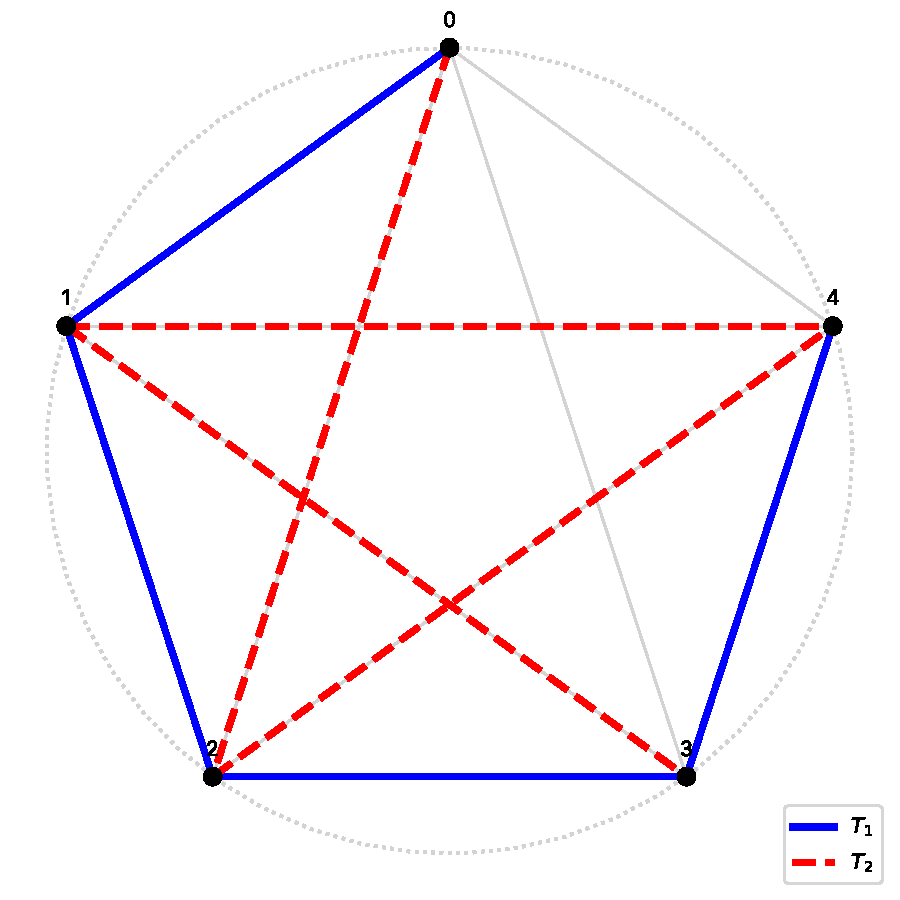
\includegraphics[width=0.85\columnwidth]{figs/spanning.pdf}
\caption{Edge-disjoint spanning trees $T_1$, $T_2$ of $K_5$}
\label{fig:q36}
\end{figure}

%---------------------------------------------------------------------
\item Consider an array $A$ of integers of size $n$. The indices of $A$ run
from $1$ to $n$. An algorithm is to be designed to check whether $A$
satisfies the condition given below.
\begin{align*}
\forall i, j \in \cbrak{1, \dots, n-1} \text{ such that } i > j, \quad
\brak{A[i+1] - A[i]} > \brak{A[j+1] - A[j]}
\end{align*}
Which one of the following gives the worst case time complexity of the
fastest algorithm that can be designed for the problem?
\hfill (CS2 2026)
\begin{multicols}{4}
\begin{enumerate}[label=\roman*)]
  \item $\Theta(n)$
  \item $\Theta(\log(n))$
  \item $\Theta(n\log(n))$
  \item $\Theta(n^2)$
\end{enumerate}
\end{multicols}
\solution Let $d_i = A[i+1] - A[i]$. The condition is
\begin{align}
d_1 < d_2 < \dots < d_{n-1}
\end{align}
which needs only the consecutive checks $d_i < d_{i+1}$: one pass, $O(n)$.
Every element must be read, since changing an unread element could break
the condition, so $\Omega(n)$ is needed. The answer is option i).

The following code implements the $O(n)$ check.
\begin{lstlisting}
codes/check.c
\end{lstlisting}

%---------------------------------------------------------------------
\item Consider a table $T$, where the elements $T[i][j]$,
$0 \le i, j \le n$, represent the cost of the optimal solutions of
different subproblems of a problem that is being solved using a dynamic
programming algorithm. The recursive formulation to compute the table
entries is as follows:
\begin{align}
T[0][k] &= T[k][0] = 1 && k = 0, 1, \dots, n \\
T[i][j] &= 2T[i-1][j] + 3T[i][j-1] && 1 \le i, j \le n
\label{eq:q39-rec}
\end{align}
Consider the following two algorithms to compute entries of $T$. Assume
that for both the algorithms, for all $0 \le i, j \le n$, $T[i][j]$ has
been initialized to 1.
\par\medskip\noindent\begin{minipage}{\linewidth}
\begin{lstlisting}[mathescape=true]
Algorithm $B_1$: For $i = 1, 2, \dots, n$
                   For $j = 1, 2, \dots, n$
                     $T[i][j] = 2T[i-1][j] + 3T[i][j-1]$

Algorithm $B_2$: For $s = 2, 3, \dots, 2n$
                   For $i = 1, 2, \dots, n$
                     For $j = 1, 2, \dots, n$
                       If $(i + j == s)$
                         $T[i][j] = 2T[i-1][j] + 3T[i][j-1]$
\end{lstlisting}
\end{minipage}\par\medskip
Algorithm $B_k$, $k \in \cbrak{1, 2}$ is said to be correct if and only if
it calculates the correct values of $T[i][j]$, for all $0 \le i, j \le n$,
(as per the recursive formulation) at the end of the execution of the
algorithm $B_k$. Which one of the following statements is true?
\hfill (CS2 2026)
\begin{enumerate}[label=\roman*)]
  \item Both algorithms $B_1$ and $B_2$ are correct
  \item Algorithm $B_1$ is correct, but algorithm $B_2$ is incorrect
  \item Algorithm $B_2$ is correct, but algorithm $B_1$ is incorrect
  \item Both algorithms $B_1$ and $B_2$ are incorrect
\end{enumerate}
\solution In \eqref{eq:q39-rec}, $T[i][j]$ needs $T[i-1][j]$ and
$T[i][j-1]$, and the boundary cells are already correct.
\begin{itemize}
  \item $B_1$ goes row by row: $T[i-1][j]$ is in the previous row and
  $T[i][j-1]$ is earlier in the same row. Correct.
  \item $B_2$ goes by anti-diagonal $s = i + j$: both dependencies have
  index sum $s - 1$, so they were computed in the previous pass. Every
  cell has $2 \le i + j \le 2n$. Correct.
\end{itemize}
The answer is option i).

The following code compares both algorithms with the recursive formulation.
\begin{lstlisting}
codes/dp.c
\end{lstlisting}

%---------------------------------------------------------------------
\item Consider the following 4-variable Boolean function
\begin{align*}
F(A, B, C, D) = \Sigma m\brak{0, 1, 2, 3, 8, 9, 10, 11}
\end{align*}
Consider $A$ as MSB, $D$ as LSB. Which one of the following options
represents the minimal sum of products form for the above function?

\textit{Note:} $+$ is OR operation, $.$ is AND operation, $'$ is NOT
operation
\hfill (CS2 2026)
\begin{multicols}{2}
\begin{enumerate}[label=\roman*)]
  \item $A' + B' + C' + D'$
  \item $B'$
  \item $A'.B' + A.B$
  \item $A'$
\end{enumerate}
\end{multicols}
\solution Minterms $0$--$3$ are $00CD$ ($A = 0, B = 0$) and minterms
$8$--$11$ are $10CD$ ($A = 1, B = 0$), with $C, D$ taking all values. So
\begin{align}
F = A'B' + AB' = B'
\end{align}
from \eqref{eq:bool-comb}. The answer is option ii).

The following code checks every option against the truth table.
\begin{lstlisting}
codes/bool.c
\end{lstlisting}

%---------------------------------------------------------------------
\item Consider the transmission of data bits $110001011$ over a link that
uses Cyclic Redundancy Check (CRC) code for error detection. If the
generator bit pattern is given to be $1001$, which one of the following
options shows the remainder bit pattern appended to the data bits before
transmission?
\hfill (CS2 2026)
\begin{multicols}{4}
\begin{enumerate}[label=\roman*)]
  \item $011$
  \item $101$
  \item $000$
  \item $100$
\end{enumerate}
\end{multicols}
\solution The generator has degree $r = 3$. From \eqref{eq:crc}, append
three zeros and divide by $1001$ modulo 2:
\par\medskip\noindent\begin{minipage}{\linewidth}
\begin{lstlisting}
110001011000
1001
-------------
010101011000
 1001
000111011000
   1001
000011111000
    1001
000001101000
     1001
000000100000
      1001
000000000100
\end{lstlisting}
\end{minipage}\par\medskip
The remainder is $100$. The answer is option iv).

The following code verifies the solution.
\begin{lstlisting}
codes/crc.c
\end{lstlisting}

%---------------------------------------------------------------------
\item Consider a stack $S$ and a queue $Q$. Both of them are initially
empty and have the capacity to store ten elements each. The elements 1, 2,
3, 4, and 5 arrive one by one, in that order. When an element arrives, it
is assigned either to $S$ (pushed on $S$) or to $Q$ (enqueued to $Q$). Once
all the five elements are stored, the output is generated in two steps.
First, stack $S$ is emptied by popping all elements. Then queue $Q$ is
emptied by dequeueing all elements. The output obtained by following this
process is $4\ 3\ 1\ 2\ 5$.

Given the output, the objective is to predict whether an element was
assigned to $S$ or $Q$. Which of the following options is/are possible
valid assignment(s) of the elements?

\textit{Note:} In the options, the notation $xS$ denotes that element $x$
was assigned to $S$ and $yQ$ denotes that element $y$ was assigned to $Q$.
\hfill (CS2 2026)
\begin{multicols}{2}
\begin{enumerate}[label=\roman*)]
  \item $1S, 2Q, 3S, 4S, 5Q$
  \item $1Q, 2Q, 3S, 4S, 5Q$
  \item $1Q, 2Q, 3Q, 4S, 5S$
  \item $1S, 2S, 3S, 4Q, 5Q$
\end{enumerate}
\end{multicols}
\solution From \ref{fm:stack-queue}, the stack's elements come out in
decreasing order and the queue's in increasing order. So the output must
be a decreasing part (stack) followed by an increasing part (queue).
\begin{table}[H]
\centering
\begin{tabular}{|c|c|c|}
\hline
\textbf{Stack} & \textbf{Queue} & \textbf{Valid?} \\
\hline
$4$ & $3\ 1\ 2\ 5$ & No \\
$4\ 3$ & $1\ 2\ 5$ & Yes: option ii) \\
$4\ 3\ 1$ & $2\ 5$ & Yes: option i) \\
$4\ 3\ 1\ 2$ & $5$ & No \\
\hline
\end{tabular}
\caption{Possible splits of the output}
\end{table}
Option iii) would output $5$ first and option iv) would output
$3\ 2\ 1\ 4\ 5$. The answer is options i) and ii).

The following code tries all 32 assignments and prints the valid ones.
\begin{lstlisting}
codes/stackqueue.c
\end{lstlisting}

%---------------------------------------------------------------------
\item Consider three processes P1, P2, and P3 running identical code, as
shown in the pseudocode below. A and B are two binary semaphores
initialized to 1 and 0, respectively. X is a shared variable initialized to
0. Each line in the pseudocode is executed atomically.

\par\medskip\noindent\begin{minipage}{\linewidth}
\centering Pseudocode of P1, P2, and P3
\begin{lstlisting}[xleftmargin=0.3\linewidth, xrightmargin=0.3\linewidth]
Wait(A);
Print(*);
X = X+1;
If (X == 2)
   {
      Print($);
      Signal(B);
   }
Signal(A);
Wait(B);
Print(#);
Signal(B);
\end{lstlisting}
\end{minipage}\par\medskip
Assume that any of the three processes can start to execute first and
context switching can happen between these processes at any arbitrary time
and in any arbitrary order. Which of the following patterns is/are possible
to be generated as an outcome of the execution of these three processes?
\hfill (CS2 2026)
\begin{multicols}{4}
\begin{enumerate}[label=\roman*)]
  \item \texttt{**\$*\#\#\#}
  \item \texttt{**\$\#*\#\#}
  \item \texttt{**\$\#\#*\#}
  \item \texttt{***\$\#\#\#}
\end{enumerate}
\end{multicols}
\solution From \eqref{eq:sem-wait} and \eqref{eq:sem-signal}, $A$ gives
mutual exclusion, so the second process to enter prints \texttt{\$} right
after its \texttt{*}, before releasing $A$. Every output therefore starts
with \texttt{**\$}, which rules out iv). \texttt{Signal(B)} after
\texttt{\$}, and after each \texttt{\#}, lets the waiting processes print
their \texttt{\#} one at a time. The third process can enter at any time
after $A$ is released: before any \texttt{\#} (option i), after one
(option ii) or after two (option iii). The answer is options i), ii) and
iii).

The following code explores every interleaving and lists all possible outputs.
\begin{lstlisting}
codes/semaphore.py
\end{lstlisting}

%---------------------------------------------------------------------
\item Consider the digital circuit shown in \figref{fig:q59-ckt} with two
input lines A and B, two select lines S0 and S1, and an output line Y. The
blocks Q and M represent active high 2:4 decoder and 4-to-1 multiplexer,
respectively. Out of 16 possible input combinations, the number of
combinations that produce Y=1 is \underline{\hspace{1.5cm}}.
(\textit{answer in integer})

\textit{Note:} One input combination is an instance of [A B S1 S0].
\hfill (CS2 2026)
\begin{figure}[H]
\centering
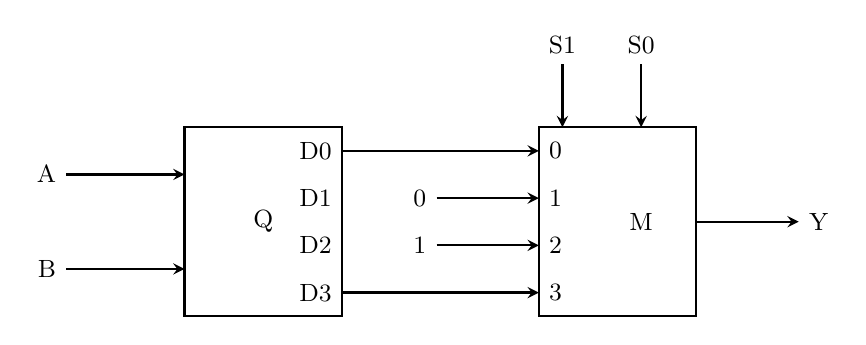
\begin{tikzpicture}[>=stealth, thick, font=\small]
  \draw (0,0) rectangle (2,2.4);
  \node at (1,1.2) {Q};
  \node[anchor=east] at (2,2.1) {D0};
  \node[anchor=east] at (2,1.5) {D1};
  \node[anchor=east] at (2,0.9) {D2};
  \node[anchor=east] at (2,0.3) {D3};
  \draw[->] (-1.5,1.8) node[left] {A} -- (0,1.8);
  \draw[->] (-1.5,0.6) node[left] {B} -- (0,0.6);
  \draw (4.5,0) rectangle (6.5,2.4);
  \node at (5.8,1.2) {M};
  \node[anchor=west] at (4.5,2.1) {0};
  \node[anchor=west] at (4.5,1.5) {1};
  \node[anchor=west] at (4.5,0.9) {2};
  \node[anchor=west] at (4.5,0.3) {3};
  \draw[->] (2,2.1) -- (4.5,2.1);
  \draw[->] (3.2,1.5) node[left] {0} -- (4.5,1.5);
  \draw[->] (3.2,0.9) node[left] {1} -- (4.5,0.9);
  \draw[->] (2,0.3) -- (4.5,0.3);
  \draw[->] (4.8,3.2) node[above] {S1} -- (4.8,2.4);
  \draw[->] (5.8,3.2) node[above] {S0} -- (5.8,2.4);
  \draw[->] (6.5,1.2) -- (7.8,1.2) node[right] {Y};
\end{tikzpicture}
\caption{Decoder and multiplexer circuit}
\label{fig:q59-ckt}
\end{figure}
\solution From \eqref{eq:decoder} and \eqref{eq:mux}, with $I_0 = D_0$,
$I_1 = 0$, $I_2 = 1$, $I_3 = D_3$,
\begin{align}
Y = S_1'S_0'\,A'B' + S_1 S_0' + S_1 S_0\,AB
\end{align}
\begin{table}[H]
\centering
\begin{tabular}{|c|c|c|}
\hline
$S_1 S_0$ & $Y = 1$ when & \textbf{Count} \\
\hline
$00$ & $A = B = 0$ & 1 \\
$01$ & never & 0 \\
$10$ & always & 4 \\
$11$ & $A = B = 1$ & 1 \\
\hline
\end{tabular}
\caption{Combinations with $Y = 1$}
\end{table}
So $6$ combinations give $Y = 1$.

The following code prints the truth table and counts $Y = 1$.
\begin{lstlisting}
codes/circuit.c
\end{lstlisting}

%---------------------------------------------------------------------
\item Consider the following ANSI-C program.
\par\medskip\noindent\begin{minipage}{\linewidth}
\begin{lstlisting}[language=C]
#include <stdio.h>
int main(){
    int *ptr, a, b, c;
    a=5; b=11; c=20;
    ptr=&a; *ptr=c; ptr=&c;
    a=*(&b); c=*ptr-a;
    printf("%d",c);
    return(0);
}
\end{lstlisting}
\end{minipage}\par\medskip
The output of this program is \underline{\hspace{1.5cm}}.
(\textit{answer in integer})

\textit{Note:} Assume that the program compiles and runs successfully.
\hfill (CS2 2026)

\solution Using \eqref{eq:deref} for \texttt{a=*(\&b)}:
\begin{table}[H]
\centering
\begin{tabular}{|l|c|c|c|c|}
\hline
\textbf{Statement} & \texttt{a} & \texttt{b} & \texttt{c} & \texttt{ptr} \\
\hline
\texttt{a=5; b=11; c=20;} & 5 & 11 & 20 & -- \\
\texttt{ptr=\&a; *ptr=c;} & 20 & 11 & 20 & \texttt{\&a} \\
\texttt{ptr=\&c;} & 20 & 11 & 20 & \texttt{\&c} \\
\texttt{a=*(\&b);} & 11 & 11 & 20 & \texttt{\&c} \\
\texttt{c=*ptr-a;} & 11 & 11 & 9 & \texttt{\&c} \\
\hline
\end{tabular}
\caption{Trace}
\end{table}
The output is $9$.

The following code verifies the solution.
\begin{lstlisting}
codes/q60.c
\end{lstlisting}

%---------------------------------------------------------------------
\item Consider the following ANSI-C function.
\par\medskip\noindent\begin{minipage}{\linewidth}
\begin{lstlisting}[language=C]
int func(int start, int end){
    int length=end+1-start;
    if((length<1)||(start<0)||(end<0)){ return(0); }
    if(length%3==0){
        return(func(start+1, end));
    } else if(length%3==1){
        return(1+func(start, end-1));
    } else {
        return(func(start+2, end));
    }
}
\end{lstlisting}
\end{minipage}\par\medskip
The maximum possible value that can be returned from this function is
\underline{\hspace{1.5cm}}. (\textit{answer in integer})

\textit{Note:} Ignore syntax errors (if any) in the function.
\hfill (CS2 2026)

\solution Let $L = \texttt{end} + 1 - \texttt{start}$. The three cases give
\begin{align}
L \equiv 0 \pmod 3 &\implies L \to L - 1 \equiv 2, \text{ adds } 0 \\
L \equiv 1 \pmod 3 &\implies L \to L - 1 \equiv 0, \text{ adds } 1 \\
L \equiv 2 \pmod 3 &\implies L \to L - 2 \equiv 0, \text{ adds } 0
\end{align}
Once $L \equiv 0$ or $2$, it never becomes $\equiv 1$ again, and the
recursion ends with $0$. So $1$ can be added at most once, for example
\begin{align}
\texttt{func(0, 0)} = 1 + \texttt{func(0, -1)} = 1
\end{align}
The maximum is $1$.

The following code searches all \texttt{start}, \texttt{end} in $[-5, 299]$ for the maximum.
\begin{lstlisting}
codes/func.c
\end{lstlisting}

%---------------------------------------------------------------------
\item The determinant of a $4 \times 4$ matrix A is 3. The value of the
determinant of 2A is \underline{\hspace{1.5cm}}. (\textit{answer in
integer})
\hfill (CS2 2026)

\solution From \eqref{eq:det-scale},
\begin{align}
\det\brak{2\vec{A}} = 2^4 \times 3 = 48
\end{align}

The following code verifies the solution with a random matrix.
\begin{lstlisting}
codes/det.py
\end{lstlisting}

%---------------------------------------------------------------------
\item Suppose an unbiased coin is tossed 6 times. Each coin toss is
independent of all previous coin tosses. Let $E_1$ be the event that among
the second, fourth, and sixth coin tosses, there are at least two heads.
Let $E_2$ be the event that among the first, second, third, and fifth coin
tosses, there are equal number of heads and tails. The conditional
probability $\pr{E_1 \mid E_2}$ is equal to \underline{\hspace{1.5cm}}.
(\textit{rounded off to one decimal place})
\hfill (CS2 2026)

\solution Let $X_i = 1$ if toss $i$ is a head and $0$ otherwise, with
$\pr{X_i = 1} = \pr{X_i = 0} = \frac{1}{2}$. Define
\begin{align}
S_1 &= X_2 + X_4 + X_6 && \text{(heads among tosses 2, 4, 6)} \\
S_2 &= X_1 + X_2 + X_3 + X_5 && \text{(heads among tosses 1, 2, 3, 5)}
\end{align}
Then $E_1 = \cbrak{S_1 \ge 2}$ and $E_2 = \cbrak{S_2 = 2}$. From
\eqref{eq:cond-prob},
\begin{align}
\pr{E_1 \mid E_2} = \frac{\pr{S_1 \ge 2,\ S_2 = 2}}{\pr{S_2 = 2}}
\label{eq:q63-cond}
\end{align}

\textbf{Joint Z-transform.} Each toss adds to $S_1$, $S_2$ or both:
\begin{table}[H]
\centering
\renewcommand{\arraystretch}{1.5}
\begin{tabular}{|c|c|c|}
\hline
\textbf{Toss} & \textbf{Adds to} & $M_{X_i}$ \textbf{in} $\brak{z_1, z_2}$ \\
\hline
2 & $S_1$ and $S_2$ & $\frac{1}{2} + \frac{1}{2} z_1^{-1} z_2^{-1}$ \\
4, 6 & $S_1$ only & $\frac{1}{2} + \frac{1}{2} z_1^{-1}$ \\
1, 3, 5 & $S_2$ only & $\frac{1}{2} + \frac{1}{2} z_2^{-1}$ \\
\hline
\end{tabular}
\caption{Contribution of each toss}
\label{tab:q63-tosses}
\end{table}
using \eqref{eq:ztrans-bern} for each toss. The tosses are independent, so
from \eqref{eq:ztrans-joint-prod},
\begin{align}
M_{S_1,S_2}\brak{z_1, z_2}
= \brak{\frac{1 + z_1^{-1} z_2^{-1}}{2}}
\brak{\frac{1 + z_1^{-1}}{2}}^{2}
\brak{\frac{1 + z_2^{-1}}{2}}^{3}
\label{eq:q63-M}
\end{align}

\textbf{Extracting $S_2 = 2$.} From \eqref{eq:ztrans-joint}, the terms of
\eqref{eq:q63-M} containing $z_2^{-2}$ give $\pr{S_1 = k, S_2 = 2}$. Expanding
\begin{align}
\brak{\frac{1 + z_2^{-1}}{2}}^{3}
= \frac{1}{8}\brak{1 + 3z_2^{-1} + 3z_2^{-2} + z_2^{-3}}
\end{align}
a factor $z_2^{-2}$ arises in two ways:
\begin{itemize}
  \item toss 2 is a tail (the $\frac{1}{2}$ term) and two of tosses
  1, 3, 5 are heads (the $\frac{3}{8} z_2^{-2}$ term);
  \item toss 2 is a head (the $\frac{1}{2} z_1^{-1} z_2^{-1}$ term) and one
  of tosses 1, 3, 5 is a head (the $\frac{3}{8} z_2^{-1}$ term).
\end{itemize}
So the coefficient of $z_2^{-2}$ is
\begin{align}
G\brak{z_1} &= \brak{\frac{1}{2}\cdot\frac{3}{8}
+ \frac{1}{2}\cdot\frac{3}{8}\, z_1^{-1}}
\brak{\frac{1 + z_1^{-1}}{2}}^{2}
= \frac{3}{64}\brak{1 + z_1^{-1}}^{3} \\
&= \frac{3}{64}\brak{1 + 3z_1^{-1} + 3z_1^{-2} + z_1^{-3}}
= \sum_{k=0}^{3} \pr{S_1 = k, S_2 = 2}\, z_1^{-k}
\label{eq:q63-G}
\end{align}

\textbf{Result.} Setting $z_1 = 1$ in \eqref{eq:q63-G} adds all the
coefficients:
\begin{align}
\pr{S_2 = 2} = G(1) = \frac{3}{64}\cdot 8 = \frac{3}{8}
\end{align}
and the coefficients of $z_1^{-2}$ and $z_1^{-3}$ give
\begin{align}
\pr{S_1 \ge 2,\ S_2 = 2} = \frac{3}{64}\brak{3 + 1} = \frac{3}{16}
\end{align}
Substituting in \eqref{eq:q63-cond},
\begin{align}
\pr{E_1 \mid E_2} = \frac{3/16}{3/8} = \frac{1}{2} = 0.5
\end{align}
Note that $\frac{G\brak{z_1}}{G(1)} = \brak{\frac{1 + z_1^{-1}}{2}}^{3}$:
given $E_2$, $S_1$ has the binomial$\brak{3, \frac{1}{2}}$ PMF of
\eqref{eq:binom-pmf}, as if toss 2 were still a fair coin.

The following code computes the joint Z-transform \eqref{eq:q63-M} as a coefficient array, extracts $G\brak{z_1}$, and checks the result by simulation in \figref{fig:q63}, where $K = S_1$ given $E_2$.
\begin{lstlisting}
codes/coins.py
\end{lstlisting}
\begin{figure}[H]
\centering
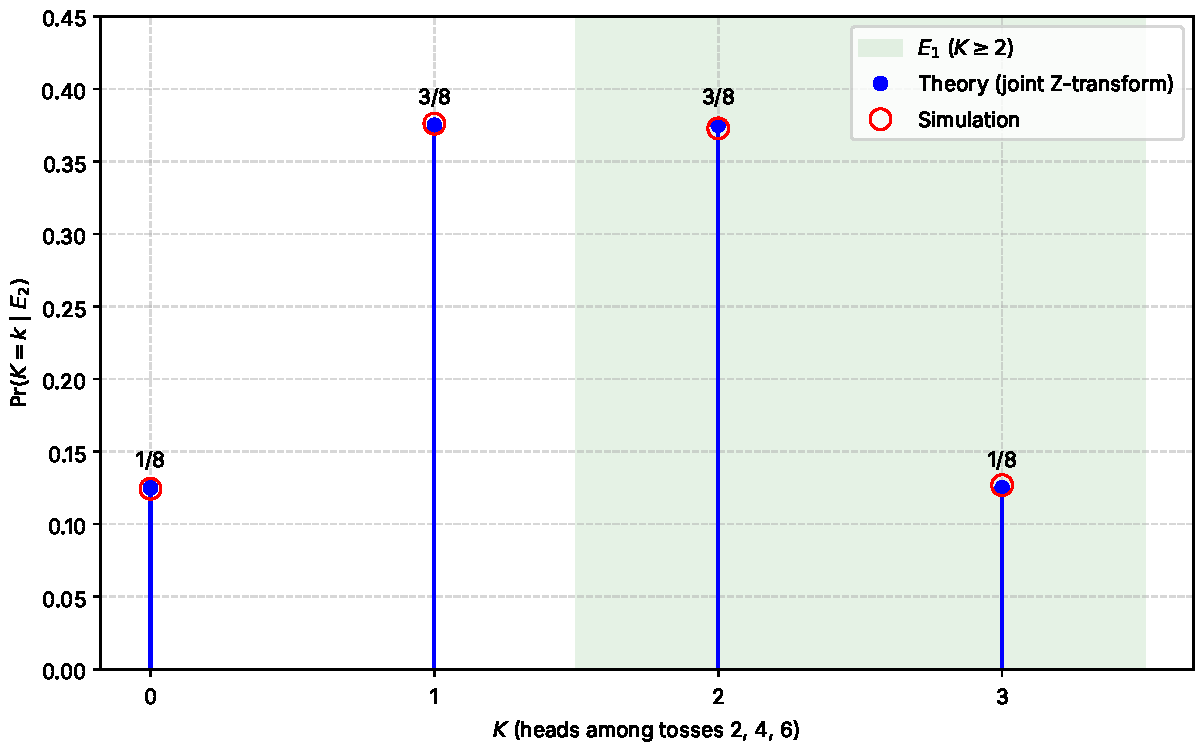
\includegraphics[width=0.85\columnwidth]{figs/coins.pdf}
\caption{PMF of $K$ given $E_2$}
\label{fig:q63}
\end{figure}

%---------------------------------------------------------------------
\item Consider a function $f : (0,1) \to \cbrak{0, 1}$ defined as follows.
For a real number $r \in (0,1)$, $f(r) = 1$ if the second digit after the
decimal point in $r$ is one of the four digits 2, 3, 6 and 7. Otherwise,
$f(r)$ is equal to 0. The number of points in $(0,1)$ at which $f$ is
discontinuous is \underline{\hspace{1.5cm}}. (\textit{answer in integer})
\hfill (CS2 2026)

\solution From \eqref{eq:digit2}, $f$ is constant on each
$\left[\frac{k}{100}, \frac{k+1}{100}\right)$, so it can only jump at
$r = \frac{k}{100}$, $k = 1, \dots, 99$, where the digit changes from
$d - 1$ to $d = k \bmod 10$ (from $9$ to $0$ when $d = 0$).
\begin{table}[H]
\centering
\begin{tabular}{|c|cccccccccc|}
\hline
$d$ & 0 & 1 & 2 & 3 & 4 & 5 & 6 & 7 & 8 & 9 \\
\hline
$f$ & 0 & 0 & 1 & 1 & 0 & 0 & 1 & 1 & 0 & 0 \\
\hline
Jump & No & No & Yes & No & Yes & No & Yes & No & Yes & No \\
\hline
\end{tabular}
\caption{Jumps of $f$}
\end{table}
$f$ jumps when $k \bmod 10 \in \cbrak{2, 4, 6, 8}$, which happens
$4 \times 10 = 40$ times for $k = 1, \dots, 99$. So $f$ has $40$ points of
discontinuity.

The following code counts the jumps and plots $f$ in \figref{fig:q64}.
\begin{lstlisting}
codes/digit.py
\end{lstlisting}
\begin{figure}[H]
\centering
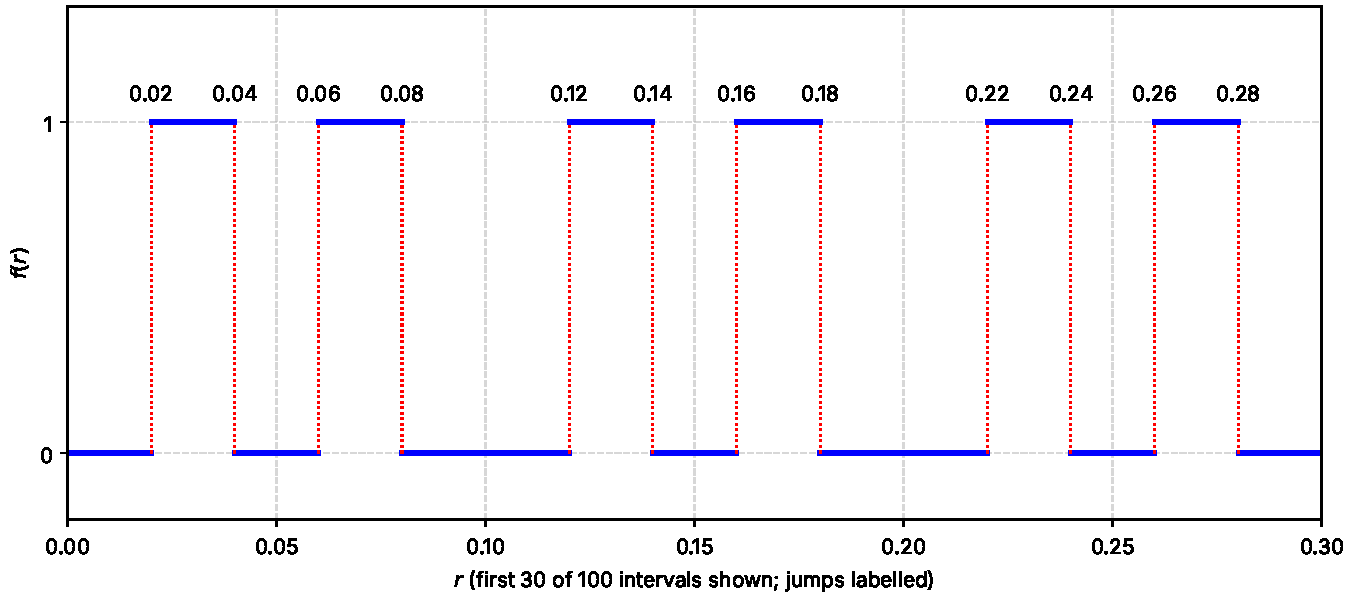
\includegraphics[width=0.85\columnwidth]{figs/digit.pdf}
\caption{$f(r)$ near the start of $(0, 1)$}
\label{fig:q64}
\end{figure}

\end{enumerate}
